\usetikzlibrary{positioning,intersections,through,backgrounds,fit}

\newcommand{\rowstyle}[1]{\gdef\currentrowstyle{#1}%
	#1\ignorespaces
}
\newcolumntype{$}{>{\global\let\currentrowstyle\relax}}
\newcolumntype{^}{>{\currentrowstyle}}

\newenvironment{addtable}
{%
	\newcommand{\binone}{Number 1}
	\newcommand{\bintwo}{Number 2}
	\newcommand{\bincar}{Carry}
	\newcommand{\binsum}{\rowstyle{\bfseries} Sum}
	\newcommand{\divrule}{\midrule}
	\begin{tabular}
		{$r|^c^c^c^c^c^c^c^c}%
		}
		{%
	\end{tabular}%
}

\newcommand{\tikzfulladder}{
	\begin{circuitikz}
		\draw node (origin) {}

		node[xor port,right=of origin] (xorone){}
		node[xor port,right=of xorone, anchor=in 1] (xortwo){}
		coordinate (xorxormidway) at ($(xorone)!.5!(xortwo)$)
		node[and port,below=of xorxormidway] (andone) {}
		node[and port,below=of andone] (andtwo) {}
		coordinate (andandmidway) at ($(andone)!.5!(andtwo)$)
		node[or port,right=of andandmidway] (or) {}


		node (A) at ([xshift=-15mm]xorone.in 1) {}
		node (B) at ([xshift=-15mm]xorone.in 2) {}

		([xshift=10mm]A.east) node[circ] {} |-(andtwo.in 1)
		([xshift=5mm]B.east) node[circ] {} |-(andtwo.in 2)

		coordinate (andoneintop) at ($(andone.in 1)!.5!(xortwo.in 2)$);

		\draw node (C) at (B |- andoneintop) {C}

		(A) node {A}
		(B) node {B}

		(A.east) |-(xorone.in 1)
		(B.east) |-(xorone.in 2)

		(C.east) -|(andone.in 1)
		(C.east) -| (andone.in 1)  node[circ,pos=0.5] {} |-(xortwo.in 2)

		(xorone.out) node[circ] {} -- (xortwo.in 1)
		(xorone.out) |- (andone.in 2)

		(andone.out) -- ++(right: 3mm) |- (or.in 1)
		(andtwo.out) -- ++(right: 3mm) |- (or.in 2)

		(or.out) -- ++(right:15mm) node[right] {Carry}
		(xortwo.out) -- ++(right:15mm) node[right] {Sum}
		;
	\end{circuitikz}
}

\chapter{Computer Architecture and Network Systems}
\section{Session One}\label{sec:session_one}

This course is for uncovering how computers work individually and together as networks.
``Stay high level when you can, but go low level when you must''

All teaching will be done solo via recordings with live sessions saved for tutorials, group discussions and labs.
The live lessons will be \(1\) hour of teaching with \(1\) hour of time to review for the next lesson.

\subsection{Assessments}\label{sub:assessments}

\begin{itemize}
    \item \(\mathbf{60\%}\): Online written exam with date TBA
    \item \(\mathbf{10\%}\) \textbf{total}: All classroom tests (roughly \(1\) test per unit)
    \item \(\mathbf{20\%}\) \textbf{total}: Two assessed exercises (\(1\) for architecture, \(1\) for networks)
    \item \(\mathbf{10\%}\) \textbf{total}: Short quizzes from most live lessons
\end{itemize}

\subsection{Group Work and Peer Learning}\label{sub:group_work_and_peer_learning}

Sometimes group work is good, sometimes it isn't; you should find your own balance.
Consider ``think, pair, share''.

\section{Session 2}\label{sec:session_2}

\subsection{Introduction to Computer Systems}\label{sub:introduction_to_computer_systems}

There are many types of computer systems:

\begin{itemize}
	\item \textbf{Servers:} Perform a few large tasks for many users. Has lots of processor power and memory.
	\item \textbf{Personal Computers:} Must balance cost and performance. Does many different tasks for just one user.
	\item \textbf{Mobile:} Highly integrated (there are multiple chips combined together like GPS and GPUs), but must be low power. Performs one program at a time for one user.
	\item \textbf{Embedded:} \emph{Very} task specific (sensing, media playback, etc.). Must be very low power. Runs one program.
\end{itemize}

\subsubsection{The Goal of Computer Systems}\label{ssub:the_goal_of_computer_systems}

A computer system should implement what we want to do with what equipment we have.
\emph{What we want to do} is have a usable computer system supporting programming and applications (which are interfaces humans can work with).
\emph{What we have} is digital electronics (which humans cannot use directly).

\subsubsection{Complexity}\label{ssub:complexity}

There is a huge difference between the individual components and the usable system since computers have billions of components.
We use \emph{abstraction} to make these components easier for us humans to use.

\begin{enumerate}
	\item Applications like Firefox
	\item Programming languages and compilers
	\item Operating systems and system software
	\item Instruction set architecture (ISA) or \emph{computer architecture}
	\item Micro-architecture which is the implementation of the ISA in hardware or the computer's organisation
	\item Digital circuits like AND, OR and NOT gates
	\item Electrons
\end{enumerate}

\subsubsection{Instruction Set Architecture}\label{ssub:instruction_set_architecture}

The \emph{Instruction set architecture} is the machine language executed by the hardware and is the interface between the circuits and the software.
The ISA must be simple enough that it can be translated directly to logic gates, but must be complex enough that high level languages can be translated to it.

\subsubsection{Operating Systems}\label{ssub:operating_systems}

An operating system provides system services -- like file handling, networking, threads and processes -- that are needed by applications and are too complex to implement directly in hardware.

\subsection{The Analogue and Digital Representation of Data}\label{sub:the_analogue_and_digital_representation_of_data}

Computers work with and manipulate data by handling and manipulating electrons.

\subsubsection{Data Representation}\label{ssub:data_representation}

Every single data type is always represented using electrons.
Storing different voltages along a wire is the act of storing data.

\subsubsection{Analogue}\label{ssub:analogue}

The analogue storing of data was only ever used briefly.
When storing data in a analogue system is where various predefined voltages represent different values.

\medskip
\begin{minipage}[t]{0.45\linewidth}
	Pros:
	\begin{itemize}
		\item Can be very fast (you don't have to worry about different bytes); old military aircraft used analogue systems for their on-board computers.
	\end{itemize}
\end{minipage}
\hfill
\begin{minipage}[t]{0.45\linewidth}
	Cons:
	\begin{itemize}
		\item There is limited precision and after many calculations, errors will have accumulated
		\item It is hard to represent data other than real numbers like integers or strings
	\end{itemize}
\end{minipage}

\subsubsection{Digital}\label{ssub:digital}

Digital data encoding is where one specific voltage represents one single value.

\medskip
\begin{minipage}[t]{0.45\linewidth}
	Pros:
	\begin{itemize}
		\item Good immunity to noise (\(4.7\)V is still considered \(5\)V)
		\item Errors do not accumulate
		\item All data types can be represented
	\end{itemize}
\end{minipage}
\hfill
\begin{minipage}[t]{0.45\linewidth}
	Cons:
	\begin{itemize}
		\item Sampling may cause a loss of data
		\item More processing can be required
	\end{itemize}
\end{minipage}

\begin{note}
	Note: To recover the analogue data from a digital signal, take note of the peaks and troughs of the digital signal and pass a sinusoidal pave through these points.
\end{note}

\subsection{Bits and Bytes}\label{sub:bits_and_bytes}

A \emph{byte} is made of eight bits where a bit is a single on or off value.
A byte is represented by \(8\) copies of the basic storage unit.

\subsubsection{Information Capacity}\label{ssub:information_capacity}

There are \(2^8\) different possible values representable by \(1\) bytes.
This can be generalised to \(V=2^{n}\) where \(V\) is the total number of values and \(n\) is the number of bits.

\subsubsection{Words}\label{ssub:words}

A word is a collection of bits in any quantity, but usually in sizes of the powers of \(2\).
There are some definitions that are usually followed (but not always):

\begin{itemize}
	\item \textbf{Short Word:} \(16 \textrm{bits} = 65536 \textrm{ values}\)
	\item \textbf{Word:} \(32 \textrm{bits} = 4294967296 \textrm{ values}\)
	\item \textbf{Long Word:} \(64 \textrm{bits} = 1.84 \times 10^{19} \textrm{ values}\)
\end{itemize}

The term ``\(64\) bit architecture'' means that the internal architecture is using (mostly) \(64\) bit words.
Generally the larger the system's word size the more performant the system since you would need \(2\) instructions to add \(2\) \(64\) bit numbers on a \(32\) bit system.

\section{Binary Numbers}\label{sec:binary_numbers}

Binary doesn't just represent data or control information, it can represent different numbers.

There are several different encodings for storing numbers in a binary system.
\begin{itemize}
	\item \textbf{Positive integers:} binary
	\item \textbf{Negative integers:} two's complement
	\item \textbf{Reals:} approximately stored using floating point representation
\end{itemize}

\begin{note}
	Note: The binary encoding system (ie.\ not two's complement) cannot represent negative numbers.
\end{note}

The \emph{least significant bit} (LSB) is the right-most bit.
The \emph{most significant bit} (MSB) is the left-most bit

\subsection{Decimal to Binary Conversion}\label{sub:decimal_to_binary_conversion}

\begin{enumerate}
	\item Check if the decimal number fits in the number of bits you have allocated using \(V=2^n\).
	\item Subtract the largest power of \(2\) you can and set that power of \(2\) to \(1\) in your binary table.
	\item Repeat until complete.
\end{enumerate}

\section{Binary Addition}\label{sec:binary_addition}

Simply add the \(0\)s and the \(1\)s together as in the example below.

\begin{figure}[H]
	\centering
	\begin{tabular}{ccc|cc|c}
		\toprule
		\(x\) & \(y\) & \(z\) & Carry & Sum & Decimal \\
		\midrule
		0     & 0     & 0     & 0     & 0   & 0       \\
		0     & 0     & 1     & 0     & 1   & 1       \\
		0     & 1     & 0     & 0     & 1   & 1       \\
		0     & 1     & 1     & 1     & 0   & 2       \\
		1     & 0     & 0     & 0     & 1   & 1       \\
		1     & 0     & 1     & 1     & 0   & 2       \\
		1     & 1     & 0     & 1     & 0   & 2       \\
		1     & 1     & 1     & 1     & 1   & 3       \\
		\bottomrule
	\end{tabular}
	\label{tbl:bin_addition}
	\caption{Binary addition (\(x+y+z\))}
\end{figure}

To add longer \(8\) bit numbers simply repeat the process many more times.

\begin{figure}[H]
	\centering
	\begin{addtable}
		\binone & 0 & 0 & 1 & 0 & 1 & 1 & 0 & 1 \\
		\bintwo & 0 & 1 & 0 & 0 & 1 & 1 & 1 & 0 \\
		\divrule
		\bincar & 0 & 0 & 0 & 0 & 1 & 1 & 0 & 0 \\
		\rowstyle{\bfseries}
		\binsum & 0 & 1 & 1 & 1 & 1 & 0 & 1 & 1 \\
	\end{addtable}
	\label{tbl:eightbit_addition}
	\caption{\(8\) bit addition example}
\end{figure}

\section{Two's Complement}\label{sec:two_s_complement}

When we add and subtract in the decimal system, the logic used for both operations is different; this would be impractical for computers.

For two's complement to work, the number of bits used \emph{must} be specified.
Because half of the numbers used are negative, the possible range of numbers is half of that possible in the binary numbering system.
This range is defined as \(-2^{n-1} \le x \le 2^{k-1} - 1\).

To subtract two numbers, simply negate (flip the bits then add \(1\)) the subtracting number then add using the method above, ignore any overflow.

To find the positive representation of a negative number, simply negate.
An alternative method is to treat the most significant bit as a negative version of what you would expect then just add normally.

\section{Hexadecimal Notation}\label{sec:hexadecimal_notation}

Hexadecimal values can be used to represent bytes and words in a easier to understand way than a long string of \(0\)s or \(1\)s since each \(4\) bits directly corresponds to \(1\) hexadecimal character.

\begin{figure}[H]
	\centering
	\begin{tabular}{c|c|c|c}
		0001 & 1010 & 1111 & 0000 \\
		1    & A    & F    & 0
	\end{tabular}
	\label{tbl:hex_bin_comparison}
	\caption{Hexadecimal and binary comparison}
\end{figure}


\section{Using Binary To Encode Non-Numeric Data}\label{sec:using_binary_to_encode_non_numeric_data}

Numbers can be used numerically (eg.\ \(23 + 17\)) or as non-numeric data to encode information (eg.\ PA3 3BT).
Non-numeric data can represent far more things and have a greater flexibility because arithmetic operations don't need to be applied.

Just like with binary counting \(V=2^n\), but you don't have to use all values.

\subsection{ASCII}\label{sub:ascii}

The \textbf{A}merican \textbf{S}tandard \textbf{C}ode for \textbf{I}nformation \textbf{I}nterchange encodes text with \(7\) bits which are made up of \(94\) printable character and \(34\) non-printable characters.

\begin{note}
	Note: ASCII also encodes numbers, but here \(\textrm{``5''} \neq 5\).
\end{note}

\subsection{Unicode}\label{sub:unicode}

Unicode extends ASCII to \(65536\) universal characters from many different languages using \(16\) bit (\(2\) byte) words.

\subsection{Bitmaps}\label{sub:bitmaps}

Each pixel is encoded as a number representing the colour of that pixel.

\subsection{Vector Graphics}\label{sub:vector_graphics}

Vectors store instructions to draw the resultant image so can be scaled up or down infinitely.

\subsection{Words}\label{sub:words}

Although all of these encodings use binary words, the words themselves have no meaning unless we are told what type of data is encoded in them.

\section{Boolean Logic and Gates}\label{sec:boolean_logic_and_gates}

There are three basic boolean logic operators: AND (\(\land\), \(\cdot\)), OR (\(\lor\), \(\parallel\)) and NOT (\(\lnot\), \(\sim\), \(!\), \(\bar{x}\)).
Eg.\ \(A \cdot B\) is the same as \(A\) AND \(B\)
sr

\begin{note}
	Note: \(1+1=2\), but also \(1+1=1\) so context is very important.
\end{note}

A \emph{truth table} is used to define the relationship between all inputs and outputs.
For \(n\) inputs, there are \(2^{n}\) outputs.

\subsection{Logic Gates}\label{sub:logic_gates}

Switches implement specific logic functions and can be called \emph{logic gates}.
In early computers, switches were controlled by magnetic fields from coils in relays to open or close paths.
Next vacuum tubes were used.
And now, we use transistors instead.

\subsubsection{AND}\label{ssub:and}

An AND gate has an output whenever both inputs are on.

\begin{minipage}{0.45\linewidth}
	\begin{figure}[H]
		\centering
		\begin{circuitikz}
			\draw
			node[and port] (and) {}
			(and.in 1) node[anchor=east] {A}
			(and.in 2) node[anchor=east] {B}
			(and.out) node[anchor=west] {Y};
		\end{circuitikz}
		\caption{The AND logic gate}
	\end{figure}
\end{minipage}
\hfill
\begin{minipage}{0.45\linewidth}
	\begin{figure}[H]
		\centering
		\begin{circuitikz}
			\draw (0,-1) coordinate (origin) to[battery] ++(0,2) to[nos=\(A\)] ++(2,0) to[nos=\(B\)] ++(2,0) to[lamp] ++(0,-2) -- (origin);
		\end{circuitikz}
		\caption{An example of the AND gate}
	\end{figure}
\end{minipage}

\subsubsection{OR}\label{ssub:or}

The OR gate has an output whenever either of the inputs are on.

\begin{minipage}{0.45\linewidth}
	\begin{figure}[H]
		\centering
		\begin{circuitikz}
			\draw
			node[or port] (or) {}
			(or.in 1) node[anchor=east] {A}
			(or.in 2) node[anchor=east] {B}
			(or.out) node[anchor=west] {Y};
		\end{circuitikz}
		\caption{The OR logic gate}
	\end{figure}
\end{minipage}
\hfill
\begin{minipage}{0.45\linewidth}
	\begin{figure}[H]
		\centering
		\begin{circuitikz}
			\draw (0,-1) coordinate (origin) to[battery] ++(0,2) to[short,-*] ++(0.5,0) coordinate (forkpoint)%to[nos=\(A\)] ++(2,0) to[nos=\(B\)] ++(2,0) to[lamp] ++(0,-2) -- (origin);
			(forkpoint) -- ++(0,-0.5) to[nos=\(B\)] ++(2,0) -| ++(0.5,0.5) coordinate (forkjoin)
			(forkpoint) -- ++(0,0.5) to[nos=\(A\)] ++(2,0) -| (forkjoin) -- ++(0.5,0) to[lamp] ++(0,-2) -- (origin);
		\end{circuitikz}
		\caption{An example of the OR gate}
	\end{figure}
\end{minipage}

\subsubsection{NOT}\label{ssub:not}

\begin{minipage}{0.45\linewidth}
	\begin{figure}[H]
		\centering
		\begin{circuitikz}
			\draw
			node[not port] (gate) {}
			(gate.in 1) node[anchor=east] {A}
			(gate.out) node[anchor=west] {Y};
		\end{circuitikz}
		\caption{The OR logic gate}
	\end{figure}
\end{minipage}
\hfill
\begin{minipage}{0.45\linewidth}
	The output is inverted to the output.
\end{minipage}

\subsubsection{BUFFER}\label{ssub:buffer}

\begin{minipage}{0.45\linewidth}
	\begin{figure}[H]
		\centering
		\begin{circuitikz}
			\draw
			node[buffer port] (gate) {}
			(gate.in 1) node[anchor=east] {A}
			(gate.out) node[anchor=west] {Y};
		\end{circuitikz}
		\caption{The BUFFER logic gate}
	\end{figure}
\end{minipage}
\hfill
\begin{minipage}{0.45\linewidth}
	The input is exactly the same as the output.
\end{minipage}

\subsubsection{NAND}\label{ssub:nand}

\begin{minipage}{0.45\linewidth}
	\begin{figure}[H]
		\centering
		\begin{circuitikz}
			\draw
			node[nand port] (gate) {}
			(gate.in 1) node[anchor=east] {A}
			(gate.in 2) node[anchor=east] {B}
			(gate.out) node[anchor=west] {Y};
		\end{circuitikz}
		\caption{The NAND logic gate}
	\end{figure}
\end{minipage}
\hfill
\begin{minipage}{0.45\linewidth}
	The output is on, unless both inputs are on.
\end{minipage}

\subsubsection{NOR}\label{ssub:nor}

\begin{minipage}{0.45\linewidth}
	\begin{figure}[H]
		\centering
		\begin{circuitikz}
			\draw
			node[nor port] (gate) {}
			(gate.in 1) node[anchor=east] {A}
			(gate.in 2) node[anchor=east] {B}
			(gate.out) node[anchor=west] {Y};
		\end{circuitikz}
		\caption{The NOR logic gate}
	\end{figure}
\end{minipage}
\hfill
\begin{minipage}{0.45\linewidth}
	The output is on only if both inputs are off.
\end{minipage}

\subsubsection{XOR}\label{ssub:xor}

\begin{minipage}{0.45\linewidth}
	\begin{figure}[H]
		\centering
		\begin{circuitikz}
			\draw
			node[xor port] (gate) {}
			(gate.in 1) node[anchor=east] {A}
			(gate.in 2) node[anchor=east] {B}
			(gate.out) node[anchor=west] {Y};
		\end{circuitikz}
		\caption{The XOR logic gate}
	\end{figure}
\end{minipage}
\hfill
\begin{minipage}{0.45\linewidth}
	Sometimes called an exclusive OR. The output is on if only one of the inputs is on.
\end{minipage}

\section{Boolean Algebra}\label{sec:boolean_algebra}

\subsection{Operations with Constants}\label{sub:operations_with_constants}

\begin{itemize}
	\item \(\mathbf{x \cdot 0 = 0}\): ANDing any variable with \(0\) gives \(0\).
	\item \(\mathbf{x \cdot 1 = x}\): ANDing any variable with \(1\) gives the original variable.
	\item \(\mathbf{x + 0 = x}\): ORing \(x\) with \(0\) gives \(x\).
	\item \(\mathbf{x + 1 = 1}\): ORing \(x\) with \(1\) gives \(1\).
\end{itemize}

\subsection{Idempotence}\label{sub:idempotence}

\emph{Indempotence} is a characteristic where performing the same action again and again results in the same answer.
For example:

\begin{itemize}
	\item \(x + x = x\)
	\item \(x \cdot x = x\)
\end{itemize}

\subsection{Commutativity}\label{sub:commutativity}

\emph{Commutativity} is where swapping the order of the inputs results in the same output.
For example:

\begin{itemize}
	\item \(x+y=y+x\)
	\item \(x \cdot y = y \cdot x\)
\end{itemize}

\subsection{Associativity}\label{sub:associativity}

The term \emph{associativity} refers to the idea that terms can be grouped in brackets in any order.
For example:

\begin{itemize}
	\item \(x + (y + z) = (x + y) + z\)
	\item \(x \cdot (y \cdot z) = (x \cdot y) \cdot z\)
\end{itemize}

\subsection{Logical Reasoning}\label{sub:logical_reasoning}

An example question might be: ``Show two boolean expressions always have the same value''.
To answer this, you can either use a truth table to brute force the answer, or you can use boolean algebra to make the two statements equal.

\subsubsection{Example}\label{ssub:example}

\begin{minipage}{0.40\linewidth}
	\begin{circuitikz}[scale=0.75]
		\draw
		node[and port] (and) {}

		node[or port, below right=of and] (or) {}

		node at ([xshift=-5mm]and.in 1) {\(0\)}
		node at ([xshift=-5mm]and.in 2) {\(p\)}

		(and.out) |- (or.in 1)

		node at ([xshift=-5mm]or.in 2) {\(q\)}
		;
	\end{circuitikz}
\end{minipage}
\hfill
\begin{minipage}{0.57\linewidth}
	\centering
	\begin{align*}
		(0 \cdot p) + q & = (p \cdot 0) + q &  & \text{Commutative law}    \\
		(0 \cdot p) + q & = 0 + q           &  & \text{Constant operation} \\
		(0 \cdot p) + q & = q               &  & \text{Constant operation}
	\end{align*}

	\begin{circuitikz}
		\draw node {\(q\)} (0.5,0) to[short] (2, 0);

	\end{circuitikz}
\end{minipage}

\section{Combinational Circuits}\label{sec:combinational_circuits}

A ``combinational circuit'' is one that works immediately and without any clock input and are created by combining AND, OR and NOT gates.

\subsection{Deriving Boolean Expressions}\label{sub:deriving_boolean_expressions}

\begin{highlight}{An example truth table}
	\begin{figure}[H]
		\centering
		\begin{tabular}{ccc|c|c}
			\toprule
			\(A\) & \(B\) & \(C\) & \(F\) & Product term                                         \\
			\midrule
			\(0\) & \(0\) & \(1\) & \(1\) & \(\overline{A}\cdot \overline{B}\cdot C\)            \\
			\(0\) & \(1\) & \(0\) & \(1\) & \(\overline{A}\cdot B\cdot \overline{C}\)            \\
			\(1\) & \(1\) & \(1\) & \(1\) & \(A\cdot B\cdot C\)                                  \\
			\(0\) & \(0\) & \(0\) & \(0\) & \(\overline{A}\cdot \overline{B}\cdot \overline{C}\) \\
		\end{tabular}
		\label{fig:example_truth_table}
	\end{figure}
\end{highlight}

\noindent
Collect the product terms where \(F=1\) and AND them together for \(\overline{A}\cdot \overline{B}\cdot C + \overline{A}\cdot B\cdot \overline{C} +A\cdot B\cdot C\), then simplify.

\subsection{Addition and Subtraction}\label{sub:addition_and_subtraction}

Addition, subtraction and negation can all be performed by a ``ripple add'' circuit.
To add just \(2\) bits together, use a ``half adder''.
To add \(3\) bits (two numbers and a carry), use a ''full adder`` -- this is what we generally use.
In order to add \(2\) full words together, use a ``ripple add'' circuit

\subsubsection{Half Adder}\label{ssub:half_adder}

Adds \(2\) bits together.
Since the resultant output could be \(0\), \(1\) or \(2\), we need to use \(2\) bits for the output which are named ``carry'' and ``sum''.

\begin{highlight}{A half adder}
	\begin{minipage}{0.42\linewidth}
		\begin{figure}[H]
			\centering
			\begin{tabular}{ccccc}
				\toprule
				\(x\) & \(y\) & Result & Carry & Sum   \\
				\midrule
				\(0\) & \(0\) & \(0\)  & \(0\) & \(0\) \\
				\(0\) & \(1\) & \(1\)  & \(0\) & \(1\) \\
				\(1\) & \(0\) & \(1\)  & \(0\) & \(1\) \\
				\(1\) & \(1\) & \(2\)  & \(1\) & \(0\) \\
				\bottomrule
			\end{tabular}
			\label{fig:half_adder}

			\medskip
			The truth table of a half adder
		\end{figure}
	\end{minipage}
	\hfill
	\begin{minipage}{0.48\linewidth}
		\begin{figure}[H]
			\centering
			\begin{circuitikz}
				\draw
				node[and port] (and) {}
				node[xor port, below=of and] (xor) {}

				node[left=of and.in 1] (x) {\(x\)}
				node[left=of xor.in 2] (y) {\(y\)}

				(x.east) -- (and.in 1)
				(y.east) -- (xor.in 2)

				([xshift=4mm]x.east) node[circ] {} |- (xor.in 1)
				([xshift=8mm]y.east) node[circ] {} |- (and.in 2)

				(and.out) node[right] {Carry \(x \cdot y\)}
				(xor.out) node[right] {Sum \(\overline{x}\cdot y + x \cdot \overline{y}\)}
				;
			\end{circuitikz}
			\label{fig:half_adder_circuit}

			\medskip
			A half adder circuit diagram
		\end{figure}
	\end{minipage}
	\medskip
\end{highlight}

\subsubsection{Full Adder}\label{ssub:full_adder}

A ``full adder'' is used to add two binary numbers together with a carry from the addition to the left and outputs the sum and the carry where \(c = x\cdot y + y \cdot z + x\cdot z\) and \(s = x \oplus y \oplus z\)

\subsubsection{Word Addition}\label{ssub:word_addition}

To add two words together (of any size), you must use a full adder for each bit of the word with the carry output being input to the next adder's carry input.

\subsubsection{Subtraction}\label{ssub:subtraction}

To subtract, simply negate and add \(1\) to the subtracting number, then add the two numbers together.

\section{Synchronous Circuits}\label{sec:synchronous_circuits}

A \emph{synchronous circuit} uses synchronous logic (sometimes called sequential logic -- which is usually synchronous anyway -- or synchronous sequential logic -- which is the fancy correct way of saying it).
Synchronous circuits have the benefit of being able to store memory/state.


\subsection{Why use sequential logic?}\label{sub:why_use_sequential_logic_}

Consider the process:

\begin{enumerate}
    \item Multiply one bit by another
    \item Shift the bit over by one
    \item Add the bit to another bit
    \item Repeat three times
\end{enumerate}
%
A combinational circuit cannot be used to do these \(4\) steps in a sequence, since we must store the output bit after each step, so we must use sequential logic.

\subsection{Timing and Gate Delay}\label{sub:timing_and_gate_delay}

All gates and wires have a slight delay (which is caused by the finite speed of light and the reaction time of transistors) that can add up over the course of an entire circuit.
Different paths can take different amounts of time, so a \emph{clock signal} is used to synchronise all of the logic gates together.

\subsection{The Flip Flop}\label{sub:the_flip_flop}

A \emph{flip flop} is a bi-stable component which is stable in either the on or off state and provides a way to store memory to let us sequence operations together.
The flip flop introduces a whole new design paradigm.

\subsubsection{Understanding Feedback}\label{ssub:understanding_feedback}

\begin{highlight}{A flip flop}
    \begin{minipage}{0.50\linewidth}
        \begin{circuitikz}
            \draw
            node[not port] (notone) {}
            node[not port, right=of notone] (nottwo) {}
            node[right=of nottwo] (q) {\(Q\)}

            (notone.in) -- ([xshift=-5mm]notone.in) |- ([yshift=15mm]$(nottwo.out)!.5!(q)$) -- ($(nottwo.out)!.5!(q)$)
            (nottwo.out) -- (q)
            (notone.out) -- (nottwo.in);
        \end{circuitikz}
    \end{minipage}
    \hfill
    \begin{minipage}{0.40\linewidth}
        If \(Q\) is \(1\), it will always be \(1\) and if \(Q\) is ever \(0\), it will always be \(0\).
    \end{minipage}
\end{highlight}
There is one problem with this circuit though: it cannot be set or reset.
We can switch it out with some NOR and AND gates to allow for these missing features.

\begin{highlight}{A resettable flip flop}
    \begin{circuitikz}
        \draw
        node[nor port] (norone) {}
        node[nor port, below=of norone] (nortwo) {}

        node[left=of norone.in 1] (r) {Reset (\(R\))}
        node[left=of nortwo.in 2] (s) {Set \(1\) (\(S\))}

        node[right=of norone.out] (q) {Output \(Q\)}
        node[right=of nortwo.out] (qbar) {Inverted output \(\overline{Q}\)}

        (r) -- (norone.in 1)
        (s) -- (nortwo.in 2)

        (norone.out) -- (q)
        (nortwo.out) -- (qbar)

        (norone.out) node[circ] {} -- ([yshift=2mm]$(norone.out)!.5!(nortwo.out)$) -- ++(-2,0) |- (nortwo.in 1)
        (nortwo.out) node[circ] {} -- ([yshift=-2mm]$(norone.out)!.5!(nortwo.out)$) -- ++(-1.8,0) |- (norone.in 2)
        ;
    \end{circuitikz}
\end{highlight}

\subsubsection{Synchronicity with flip flops}\label{ssub:synchronicity_with_flip_flops}

Flip flops are synchronous bi-stable components.
\emph{Synchronous} means that the output changes only when a clock signal is supplied.

\subsubsection{The delay flip flop}\label{ssub:the_delay_flip_flop}

The \emph{delay flip flop} is a brand new primitive component that stores a single bit.
A DFF has a single input, a single output and a clock signal input.

Every flip flop must be connected to the same clock in order to be synchronous and the clock signal must arrive at all components at the same time.
\textbf{No logic is ever performed on the clock signal} -- it is strictly a control signal.

\subsection{Clock ticks and cycles}\label{sub:clock_ticks_and_cycles}

\emph{Ticks} are individual events in time (tick, tock, tick, \ldots).
\emph{Cycles} are the intervals between the ticks.

A flip flop will stay stable for the entire duration of a cycle.
During a cycle, all logic circuits are updated and their outputs propagate through the circuit until all of the outputs are stable at a valid value.
Only once all outputs are stable and valid can a new tick occur.

\subsubsection{Clock speed}\label{ssub:clock_speed}

\emph{Clock speed} is the rate at which the internal clock signal ticks and is measured in Hertz (Hz).
A typical processor has a clock speed on the order of magnitude \(1\)GHz which is \(1\times 10^{9}\)Hz or \(1\times 10^{-9}\) seconds per tick.
At these very fast speeds, the speed of light becomes important.

\section{The applications of flip flops}\label{sec:the_applications_of_flip_flops}

\subsection{Registers}\label{sub:registers}

A register generally words on \(8\) bit words.
In order to create an \(8\) bit register, we must use \(8\) individual flip flops together.
Registers have a CLR (clear) signal to empty all flip flops.

A \emph{bus} is a collection of signals all coming from or going to the same place.

\subsection{Finite state machines}\label{sub:finite_state_machines}

In combinational circuits, \(1\) input means \(1\) output.
In a finite state machine, the output depends on the current state as well as the current input.
After each operation, the state is updated with the current output.

An ATM is an example of a finite state machine where the machine will do different things when you put your card in depending on what screen you are on.

\section{Logic devices for a CPU}\label{sec:logic_devices_for_a_cpu}

CPUs are complex, but they are made of only a few basic components:
\begin{itemize}
	\item Registers
	\item (De)muxers
	\item ALU
	\item Others\ldots
\end{itemize}

\subsection{Register Recap}\label{sub:register_recap}

Resisters are the most common building block in a CPU and so far we have only seen the parallel types where there are \(8\) inputs and outputs.
There are also serial registers where each value is input one bit at a time, then output again one bit at a time.
We even get shift left serials; shift right serials; parallel in, serial out; serial in parallel out; and rotate left \& right registers.

\subsection{Multiplexers and Demultiplexers}\label{sub:multiplexers_and_demultiplexers}

Sometimes also called a ``data selector''.
Allows you to chose between \(2^{n}\) inputs to be output.
It is important to note that in a multiplexer there is a distinct difference between the data inputs and the control input.

\subsubsection{Input Multiplexer}\label{ssub:input_multiplexer}

The \emph{\(2\)-to-\(1\)} multiplexer has \(2\) inputs (named \(I_0\) \(I_1\)), a selector (\(S\)) and an output \(O\).
The input depends on all three inputs (\(I_0\), \(I_1\) and \(S\)).
\(O = (I_0\cdot\overline{s}) + (I_1\cdot\overline{s})\)

\begin{highlight}{A multiplexer}
	\begin{circuitikz}
		\draw
		node[and port] (andone) {}
		node[and port, below=of andone] (andtwo) {}
		node[not port, left=of andone.in 2, scale=0.6] (not) {}
		([xshift=20mm]$(andone.out)!.5!(andtwo.out)$) node[or port] (or) {}

		(not.out) -- (andone.in 2)

		([xshift=-5mm]andone.in 1) node (io) {\(I_0\)}
		([xshift=-5mm]andtwo.in 2) node (it) {\(I_1\)}

		(io.east) -- (andone.in 1)
		(it.east) -- (andtwo.in 2)

		([xshift=-30mm]andtwo.in 1) node (s) {\(S\)}
		(not.in) -- ([xshift=-5mm]not.in) coordinate (leftofnot) |- (s)
		(andtwo.in 1) -- (leftofnot |- andtwo.in 1) node[circ] {}

		(or.out) -- ++(5mm,0) node[right] {\(O\)}
		(andone.out) |- (or.in 1)
		(andtwo.out) |- (or.in 2)
		;
	\end{circuitikz}
\end{highlight}


\subsubsection{Demultiplexer}\label{ssub:demultiplexer}

A \emph{demultiplexer} basically reverses the multiplexer by letting one output get sent to one of \(2^{n}\) outputs.

\subsection{ALU}\label{sub:alu}

The arithmetic and logic unit is a combinational circuit (ie.\ it has no clock) that performs basic arithmetic (addition, subtraction, multiplication, division) and basic boolean logic (AND, OR, NOT) operations.
The results of all operations are calculated and a selection line feeding into a multiplexer lets you chose which of the many operations you want the output from.

\section{Register Transfer Unit}\label{sec:register_transfer_unit}

A register transfer unit can respond to instructions almost like a CPU does.

\subsection{Simple instructions}\label{sub:simple_instructions}

A simple instruction (sometimes named ``assembly instructions'') must:
\begin{itemize}
	\item Perform exactly \(1\) operation
	\item Be of a fixed form (size)
	\item Be limited in variety (there should only be a small number of types of statement)
\end{itemize}
%
Our RTM will have:
\begin{itemize}
	\item Assignment: \(R_2 := 6\)
	\item Add and assign: \(R_3:=R_1+R_0\)
\end{itemize}

\subsection{Register File}\label{sub:register_file}

A \emph{register file} is an array of registers which are named \(R_0\) to \(R_n\) and are addressed by the binary value of \(n\).

\begin{highlight}{A register file}
	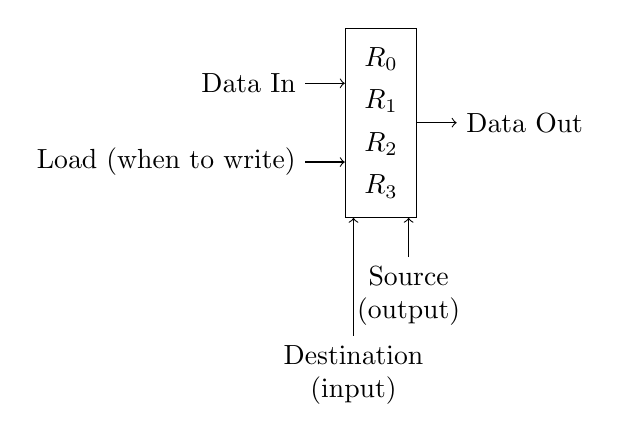
\begin{tikzpicture}
		\draw
		node (zero) {\(R_0\)}
		node[below=0mm of zero] (one) {\(R_1\)}
		node[below=0mm of one] (two) {\(R_2\)}
		node[below=0mm of two] (three) {\(R_3\)}

		node[draw,fit=(zero) (one) (two) (three)] (box) {};

		\draw[->] ([xshift=-5mm,yshift=5mm]box.west) node[left] {Data In} -- ([yshift=5mm]box.west);
		\draw[->] ([xshift=-5mm,yshift=-5mm]box.west) node[left] {Load (when to write)} -- ([yshift=-5mm]box.west);
		\draw[->] ([xshift=3.5mm,yshift=-5mm]box.south) node[below,align=center] {Source\\(output)} -- ([xshift=3.5mm]box.south);
		\draw[->] ([xshift=-3.5mm,yshift=-15mm]box.south) node[below,align=center] {Destination\\(input)} -- ([xshift=-3.5mm]box.south);
		\draw[<-] ([xshift=5mm]box.east) node[right] {Data Out} -- (box.east);
	\end{tikzpicture}
\end{highlight}

\subsubsection{Two Readouts}\label{ssub:two_readouts}

To perform an ADD or SUB operation we need an extra output because we need two operands.
Currently our input is connected to just \(1\) register but load (\(ld\)) is connected to all of the registers, so any time we trigger \(ld\), all of the registers are emptied.
We use a demuxer to chose between the registers so we only write to \(1\).

\subsubsection{ALU}\label{ssub:alu}

We add an ALU to give our RTM the ability to actually perform actions.

\subsection{Architecture}\label{sub:architecture}

The register file has two outputs and the ALU has two inputs.
For now the ALU will only ADD or SUB.
If we connect the inputs to the outputs, we will create a feedback loop such that when the clock ticks: \(reg[d] := reg[S_a] + reg[S_b]\).

We can now: load external data and load from an ALU result using a multiplexer to switch between the choices.

\begin{highlight}{The architecture of an ALU}
	\begin{tikzpicture}
		\draw
		node [draw, thick, shape=rectangle, minimum width=2cm, minimum height=3cm, anchor=center] (reg) {Register file}
		node [yshift=10mm, draw, thick, shape=rectangle, minimum width=3cm, minimum height=1cm, anchor=center,left=of reg] (mux) {Multiplexer}
		node [draw, thick, shape=rectangle, minimum width=3cm, minimum height=1cm, anchor=center,right=of reg] (alu) {ALU}
		node [draw, thick, shape=rectangle, minimum width=2cm, minimum height=1cm, anchor=center,below=of alu] (aluctl) {ALU Control}
		;

		\draw[<-] ([yshift=3mm]mux.west) -- ++ (-0.5, 0) |- ([yshift=5mm]reg.north) -| (alu.north) node[midway, above] {ALU result};
		\draw[->] ([xshift=-5mm,yshift=-3mm]mux.west) node[left] {\(x\)} -- ([yshift=-3mm]mux.west);
		\draw[->] (mux.east) -- node[above] {\(x\)} ([yshift=10mm]reg.west);
		\draw[->] ([xshift=-5mm,yshift=-10mm]reg.west) node[left] {load} -- ([yshift=-10mm]reg.west);
		\draw[->] ([yshift=2.5mm]reg.east) -- ([yshift=2.5mm]alu.west) coordinate[midway, name=midalutop];
		\draw[->] ([yshift=-2.5mm]reg.east) -- ([yshift=-2.5mm]alu.west) coordinate[midway, name=midalubottom];
		\draw[->] (aluctl.north) -- (alu.south);
		\draw[<-] (mux.south) -- ++(0,-10mm) node[below] {arith};

		\draw
		node [shape=rectangle, draw, below=of reg, minimum height=0.75cm] (sa) {\(S_a\)}
		node [shape=rectangle, draw, left=0mm of sa, minimum height=0.75cm] (d) {\(d\)}
		node [shape=rectangle, draw, right=0mm of sa, minimum height=0.75cm] (sb) {\(S_b\)}
		node [shape=rectangle, draw, left=0mm of d, minimum height=0.75cm] (op) {\(op\)}
		node [below=0mm of sa] {Instruction register}
		;

		\draw[->] (sa) -- (reg.south);
		\draw[->] (d) -- (reg.south-|d);
		\draw[->] (sb) -- (reg.south-|sb);
		\draw[->] (op) -- ++(-7mm, 0) |- ++(6,-1) node[below] (cu) {Control unit};
		\draw[->] (cu.north-|aluctl.south) node[circ] {} -- (aluctl.south);

		\draw
		(midalubottom) to[short, *-] ++(0,-0.75) -- ++(3.25,0) node[right] {\(r_a\)}
		(midalutop) to[short, *-] ++(0,0.75) -- ++(3.25,0) node[right] {\(r_b\)}
		;
	\end{tikzpicture}
\end{highlight}
%
\begin{itemize}
	\item \(x\) is the data input line
	\item \(arith\) and \(ld\) are the data inputs
	\item \(d\), \(S_a\), \(S_b\) are the address inputs to specify the target registers
\end{itemize}

\noindent
When a tick occurs the circuit runs operation that match this code:
\begin{highlight}{Operational logic of an ALU}
	\begin{code}{python}
		if ld:
		if arith:
		reg[d] := reg[sa] + reg[sb]
		else:
		reg[d] := x
	\end{code}
\end{highlight}
%
All other registers (varibles) stay unchanged.

\subsubsection{Controlling a Circuite}\label{ssub:controlling_a_circuite}

The ``core'' of any RTM circuit is a register and an adder.
To make it useful, we must use the \(arith\), \(load\) and \(op\) signals to control it.

\subsubsection{Simple RTM Programs}\label{ssub:simple_rtm_programs}

Each variable must be a register so we can assign a value to a register, or assign the result of an addition or subtraction to a register.

\section{Computer Organisation Introduction}\label{sec:computer_organisation_introduction}

\emph{Organisation} is the term used to refer to the physical circuits.
\emph{Architecture} is the term used to refer to the interface programmers can use (like instructions).

All programs have memory and data, each with their own addresses.

IO devices must use an IO module to speak to IO devices since the CPU is a very general device and is kept as simple as possible.
IO devices are \emph{memory mapped} meaning that the CPU can access certain memory addresses to tell the IO module to perform a task.

\section{Von-Neuman Machines (IAS)}\label{sec:von_neuman_machines_ias_}

Hardwired systems are inflexible (an ADDer will always ADD).
If we were to create a general system that uses control signals to do many different things we could extend a system with a new set of control signals to provide new functionality.

\subsection{IAS Machine}\label{sub:ias_machine}

There were four components that separated the IAS from computers before it:
\begin{enumerate}
    \item Memory stored both programs and data
    \item An ALU operated using binary data
    \item A control unit interprets and executes instructions from memory
    \item IO is controlled by a control unit
\end{enumerate}
%
Most computers have this architecture.
The von Neuman machine is a model saying:
\begin{itemize}
    \item There should be four main subsystems (above)
    \item Stored program concept: store programs in memory
    \item Sequential execution of instructions (fetch, decode, execute)
\end{itemize}
%
The von Neuman machines have a selection of special registers to use also:
\begin{itemize}
    \item \(PC\): Program Counter - stores the index of the current instruction
    \item \(IR\): Instruction Register - stores the current instruction
    \item \(MAR\): Memory Address Register - what memory is currently being read from
    \item \(MBR\): Memory Buffer Register - what data was just read.
    \item \(IO AR\): Input/Output Address Register - what IO memory register is currently being read from
    \item \(IO BR\): Input/Output Buffer Register - what data was just read from an IO register
\end{itemize}

\subsection{Instruction Cycle}\label{sub:instruction_cycle}

\begin{highlight}{The fetch-execute cycle}
    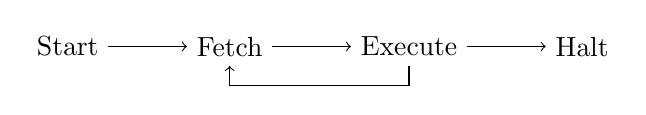
\begin{tikzpicture}
        \draw
        node (s) {Start}
        node[right=of s] (f) {Fetch}
        node[right=of f] (e) {Execute}
        node[right=of e] (h) {Halt};
        \draw[->] (s) -- (f);
        \draw[->] (f) -- (e);
        \draw[->] (e) -- (h);
        \draw[->] (e) -- ++(0,-5mm) -| (f);
    \end{tikzpicture}
\end{highlight}
\begin{enumerate}
    \item The program fetches the instruction at the program counter
    \item We increment the program counter (unless explicitly told not to when doing branches)
    \item Load the instruction to the instruction register
\end{enumerate}
%
There are four types of instruction: processor, memory; processor, IO; data processing; and control which may be combined together.

\section{The CPU}\label{sec:the_cpu}

A CPU has a set of requirements that it must meet in order to function correctly:
\begin{itemize}
	\item Fetch instructions from memory
	\item Interpret those instructions
	\item Fetch data from memory
	\item Process data
	\item Write data back to memory again
\end{itemize}

\subsection{The CPU and the System Bus}\label{sub:the_cpu_and_the_system_bus}

The system bus is made up of several smaller buses:
\begin{itemize}
	\item \textbf{Control bus}: transfers control signals
	\item \textbf{Address bus}: transfers memory addresses about
	\item \textbf{Data bus}: transfers data to and from memory
\end{itemize}

\subsection{Internal structure of a CPU}\label{sub:internal_structure_of_a_cpu}

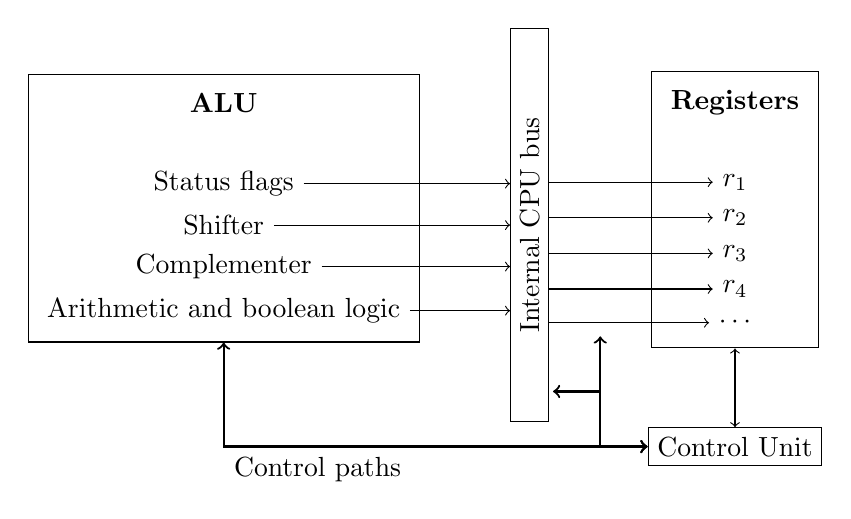
\begin{tikzpicture}
	\draw
	node (alu) {\textbf{ALU}}
	node[below=5mm of alu] (status) {Status flags}
	node[below=0mm of status] (shift) {Shifter}
	node[below=0mm of shift] (compl) {Complementer}
	node[below=0mm of compl] (abl) {Arithmetic and boolean logic}
	node[draw,fit=(alu) (status) (shift) (compl) (abl)] (alubox) {};

	\draw node [draw,shape=rectangle, minimum height=5cm, minimum width=0cm, anchor=center,right=of shift, xshift=20mm] (cpubus) {\rotatebox{90}{Internal CPU bus}};

	\draw[->] (status.east) -- (cpubus.west |- status);
	\draw[->] (shift.east) -- (cpubus.west |- shift);
	\draw[->] (compl.east) -- (cpubus.west |- compl);
	\draw[->] (abl.east) -- (cpubus.west |- abl);

	\draw
	node[right=5cm of alu] (reg) {\textbf{Registers}}
	node[below=5mm of reg] (rone) {\(r_1\)}
	node[below=0mm of rone] (rtwo) {\(r_2\)}
	node[below=0mm of rtwo] (rthree) {\(r_3\)}
	node[below=0mm of rthree] (rfour) {\(r_4\)}
	node[below=0mm of rfour] (rdots) {\(\cdots\)}
	node[draw,fit=(reg) (rone) (rtwo) (rthree) (rfour) (rdots)] (regbox) {};

	\draw[<-] (rone.west) -- (cpubus.east |- rone.west);
	\draw[<-] (rtwo.west) -- (cpubus.east |- rtwo.west);
	\draw[<-] (rthree.west) -- (cpubus.east |- rthree.west);
	\draw[<-] (rfour.west) -- (cpubus.east |- rfour.west);
	\draw[<-] (rdots.west) -- (cpubus.east |- rdots.west);

	\draw node [draw,shape=rectangle, anchor=center,below=of regbox] (cu) {Control Unit};
	\draw[<->] (cu) -- (regbox);

	\draw[<->, thick] (cu.west) -| (alubox.south) node[midway, below right] {Control paths};
	\draw[<->, thick] (cu.west) -| ++(-6mm, 14mm);
	\draw[<->, thick] (cu.west) -| ++(-6mm, 7mm) -- ++(-6mm, 0);
\end{tikzpicture}

\subsection{What does an n-bit architecture mean?}\label{sub:what_does_an_n_bit_architecture_mean_}

It means that the word size of a processor is size \(n\).
Generally this means that instructions; internal registers; internal interconnects (register bus, data bus, control bus); and the ALU can handle numbers of that size.

\section{Registers}\label{sec:registers}

\subsection{New top down perspective}\label{sub:new_top_down_perspective}

CPU must have working space -- named registers
The number and functions of registers varies between processor designs -- this is a major design decision
Registers are at the very top of the memory hierarchy (and are the fastest)

\subsection{Register Organisation}\label{sub:register_organisation}

Registers can be ``user visible'' (general purpose or specialized) and store data the user knows about.
Registers can also be for control or status which only the CPU knows about.

\subsection{User Visible}\label{sub:user_visible}

Accessible through machine language and can be general purpose or more specialised:
\begin{itemize}
	\item data(accumulator stores output of accumulated output of alu)
	\item Address (segment pointer, index regigser, stack pointer)
	\item Condition codes(flags) which are user visible, but not writeable.
\end{itemize}
There is a trade-off between general purpose and specialised because a general purpose one cannot be optimized like a specialised one can be.

\subsection{How wide?}\label{sub:how_wide_}

Large enough to hold full memory addresses and full data words.
Often is its possible to combine two registers and store one piece of large data

\subsection{Control and status registers}\label{sub:control_and_status_registers}

Generally not user visible
\begin{itemize}
	\item program counter
	\item instruction register
	\item  memory address register
	\item memory bugger register
	\item program status word
\end{itemize}

\subsubsection{Program status word}\label{ssub:program_status_word}

Stores many separate bits together which are flags (like the result of the last program)
Can be read implicitly by programs (eg. jump if \(0\))
Cannot (usually be set by programs)
Can be considered both control/status and user visible.

\section{Fetch execute cycle}\label{sec:fetch_execute_cycle}

\emph{Functional view of processor} -- what sequence of processes need to be done to do something.

\subsection{Fetch cycle}\label{sub:fetch_cycle}

\begin{itemize}
	\item Program counter stores address of next instruction to fetch
	\item Processor fetches from memory at program counter
	\item Increment program counter(unless told not to)
	\item Memory loaded into instruction register
\end{itemize}

\section{Interrupts}\label{sec:interrupts}

Is a mechanism by which other modules can interrupt the normal sequence of processing.

\begin{itemize}
	\item Program: an overflow or division by zero
	\item Timer (do something for a certain time): pre-emptive multitasking
	\item Input/output: an IO controller operates on a different time scale -- it could either wait ages for something to happen, or just get interrupted later on.
	\item Hardware failure: memory parity error
\end{itemize}

\subsection{Transfer of Control via Interrupts}\label{sub:transfer_of_control_via_interrupts}

When a user program is interrupted, the sequence of operations jumps to an interrupt handler:

\begin{center}
	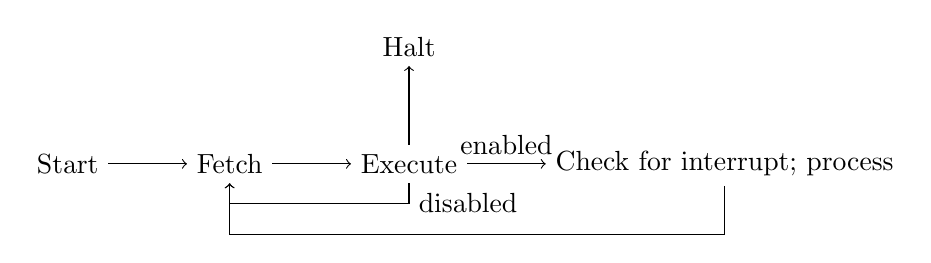
\begin{tikzpicture}
		\draw
		node (s) {Start}
		node[right=of s] (f) {Fetch}
		node[right=of f] (e) {Execute}
		node[above=of e] (h) {Halt}
		node[right=of e] (i) {Check for interrupt; process};
		\draw[->] (s) -- (f);
		\draw[->] (f) -- (e);
		\draw[->] (e) -- (h);
		\draw[->] (e) -- (i) node[above,midway] {enabled};
		\draw[->] (e) -- ++(0,-5mm) node[right] {disabled}-| (f);
		\draw[->] (i) -- ++(0,-9mm) -| (f);
	\end{tikzpicture}
\end{center}

\section{Pipe lining}\label{sec:pipe_lining}

The execution of instructions can be sped up be pipe lining.
Operations of an instruction (fetch, decode, execute, store) occur in sequence.
Each operation can be performed independently of others so all of the processing units can work simultaneously.

Pipe lining introduces parallelism into the fetch execute cycle.

\begin{note}
	In this section four operations per instruction are used (fetch, decode, execute, store). This can be different.
\end{note}

You could naively run fetch, decode, execute and store each instruction one after the other; or you could instead overlap the instructions such that after one instruction is finished fetching, another one is fetched immediately after.
This decreases the total time significantly.

\subsection{The impact on performance}\label{sub:the_impact_on_performance}

Pipe lining does \emph{not} reduce the latency of a single instruction (each individual instruction still takes the same amount of time at \(4\) cycles).

The overall throughput is increased since an instruction is finishing every cycle, instead of one only every fourth cycle, which makes throughput \(1\) cycles per instruction (CPI) instead of the \(6\) CPI.

From when the pipeline becomes full (at cycle \(4\)) there are \(4\) tasks (fetch, decode, etc.) running per cycle -- this is when there are the most performance gains.

\medskip
\noindent
In general, an \(n\) stage pipeline will improve instruction execution throughput \(n\) fold, but have no impact on the instruction latency.

We are making some assumptions here though:
\begin{itemize}
	\item There is no initial delay of filling the pipeline.
	\item All pipeline stages take exactly one unit time to complete.
	\item There are no ``hazards'' (comes up later on).
\end{itemize}

\subsection{Hazards}\label{sub:hazards}

A hazard is a conflict between different pipeline stages which stands in the way of achieving the theoretical maximum performance.

Branching means that the flow of instructions may change while the next instructions are already in the pipe line (some instructions are skipped).
We have to \emph{flush} the pipeline (remove all currently incomplete instructions), which causes \emph{branch penalties} and requires another ``initial start-up time'' to get back up to full speed.

There are three types:
\begin{enumerate}
	\item Resource hazard: two different stages need to access the same resource (memory) at the same time.
	\item Data hazard: write after read (WAR) -- not really need just something to keep in mind.
	\item Control hazard: branches, interrupts
\end{enumerate}
\section{Memory}\label{sec:memory}

\begin{itemize}
	\item In board memory (on the CPU): registers, cache, main memory
	\item Outboard storage: magnetic disk, solid state disk, flash devices, optical storage
	\item Off-line storage: Magnetic tape, DNA(?)
\end{itemize}
%
For each of these there are trade-offs to be made: capacity, performance and cost.
As capacity increase, the performance and the cost per bit comes down and as performance increases, the cost per bit does too.

As you go down the hierarchy, the cost decreases, the capacity increases and the access time increase, however the frequent of access by the CPU decreases too.

\subsection{Cache}\label{sub:cache}

A cache is a small about of very fast memory that sits on the processor itself (usually) and in between the main memory and CPU which contains a \emph{copy} of the main memory.

Multiple levels are common where there is less of the more expensive, faster memory and more of the cheaper slower memory.

Reading from cache is handled by the processor so that you only have to put a main memory address on the address bus and you will get the data from the cache if it is there.
Writing from the cache will mean that the main memory and the cache are out of sync -- to solve this you can either ``write-back'' (data is written in bulk) or ``write-through'' (data is written in real time).
This can be very tricky when you have more than one processor core accessing main memory.

\subsection{Cache overview}\label{sub:cache_overview}

\begin{enumerate}
	\item CPU requests contents from memory location
	\item Check cache for data
	      \begin{itemize}
		      \item If present: get from cache (``cache HIT'')
		      \item If not, read required block to cache in a full block (not just a single address, but a few around it because you'll likely need the addresses around it too -- ``locality of reference''), named a ``cache MISS''
	      \end{itemize}
	\item Deliver from cache to CPU
\end{enumerate}
Cache includes tags to identify which block of main memory is in each cache slot since cache is smaller than main memory and cannot store all of it.

\subsection{Cache Size}\label{sub:cache_size}

Why not have more cache to improve the chance of a cache HIT?
It costs co much more than DRAM, so cannot be too big.
Also, if cache is bigger, more gates will be involved which will make it slower.
There is no single ``optimal'' cache design.

\section{Main memory}\label{sec:main_memory}

Main memory (prefered), RAM, DRAM and internal memory all refer to the same thing.

Main memory, stores instructions and data and is made form semiconductors etched on to a silicon chip.
The name ``RAM'' comes from memory being random access, this isn't useful as many of the other memories are also random access.

\subsection{DRAM}\label{sub:dram}

Stands for dynamic RAM.
Bits are stored as a charge in a capacitor.
Charges leak so they need to be recharged even when powered.

The construction of a it is very simple, so is less expensive and simpler per bit. However, it is slower than cache and needs refresh circuits to store any data.

Used for main memory.

\subsection{Static RAM}\label{sub:static_ram}

Bits are stored as on/off switches.
There is no charge leak or refreshing needed so no refreshing circuits are needed.

This means that they also need to be more complex (using flip flops), larger and more expensive.
Cache memory generally uses SRAM so it is faster.

\subsection{Read Only Memory}\label{sub:read_only_memory}

Permanent storage (non volatile).
Stores frequently uses library subroutines.
System programs (BIOS) are stored here and loads programs into the (currently empty) system memory.

Is also random access.

\section{Computer Performance}\label{sec:computer_performance}

The amount of memory and clock speed has been increasing exponentially.
Clock speed has been increasing at a faster rate than memory capacity leading to the \emph{logic memory gap} which is one of the main processor bottlenecks.

\begin{itemize}
    \item You should increase the number of bits received at one time (make DRAM wider, not deeper because deeper is slower)
    \item Reduce frequency or memory access (have a more compelx cache and have cache on the chip).
    \item Increase interconnection bandwidth (use hierarchy of buses or increase bus speed, etc.).
\end{itemize}

\subsection{IO performance}\label{sub:io_performance}

Input and output devices are \emph{very} slow (keyboards only have \(10\)s of bits per second).
Use interrupts, multi-level bus structures and allow direct memory access.

\subsection{How to increase processor speed}\label{sub:how_to_increase_processor_speed}

\begin{itemize}
    \item Increase clock frequency by shrinking logic gates.
    \item Increase size and speed of caches
    \item Change processor organisation and architecture (parallelism)
\end{itemize}
%
Ideally all components should be able to work at their maximum performance.
Try not to let one component stall others.

\subsection{Performance Assessment}\label{sub:performance_asssessment}

\subsubsection{Clock speed}\label{ssub:clock_speed_one}

Clock speed cannot be arbitrary (ie. data should be reliably availbale at all inputs on a clock edge) so clock speed is not the whole story.

\subsubsection{Instruction execution rate}\label{ssub:instruction_execution_rate}

Average clock cycles per instruction of programs.
CPI alone won't tell us the execution time for a certain program.
We can find out number of clock ticks needed for \(n\) number of instructions, but we don't know what the duration of each clock cycle is.
\begin{align*}
    T = I_c \times CPI \times \tau
\end{align*}

\subsection{MIPS and MFLOPS}\label{sub:mips_and_mflops}

Millions of instructions per second (MIPS).
\begin{highlight}{MIPS rate formula}
    \begin{align*}
        \textrm{MIPS rate} = \frac{I_c}{T \times 10^6} = \frac{f}{CPI \times 10^6}
    \end{align*}
\end{highlight}
Millions of floating point instructions per second (MFLOPS).
Heavily dependent on instruction set, compiler design, processor implantation, cache and memory hierarchy.
MIPS and MFLOPS are bad for measuring performance.

\subsubsection{Why are the not good enough?}\label{ssub:why_are_the_not_good_enough_}

Modern processors are CISC (complex instruction set) which means one instruction can do complex tasks.
Some processors are RISC (reduced insturction set) and require several instructions per task which takes longer.

\subsection{Benchmarks}\label{sub:benchmarks}

\begin{itemize}
    \item Programs designed to test performance
    \item Written in high level languages (compile for different architectures)
    \item Represents style of task (systems, numerical, commercial)
    \item Is easily measured (probably by time)
    \item Is widely distributed and probably open source
    \item eg. System Performance Evaluation Corporation (SPEC)
\end{itemize}


\section{Instructions Introduction}\label{sec:instructions_introduction}

\subsection{Key ideas for programmable machines}\label{sub:key_ideas_for_programmable_machines}

\begin{itemize}
	\item   A machine that can perform a fixed sequence of simple arithmetic operations
	\item Provide a way to change that sequence (punch cards, code)
	\item Make it possible to compare two numbers and decide what to do next (A Babbage's Analytical Engine -- the first turing-complete machine).
\end{itemize}

\subsection{The language of machines}\label{sub:the_language_of_machines}

There are many programming languages, but each machine has its own machine language.
Each programming language is translated in to machine language by software called a compiler.

\subsection{Machine Language}\label{sub:machine_language}

Examples:
\begin{itemize}
	\item x86
	\item ARM
	\item MIPS
	\item SPARC
\end{itemize}
All are different.

\subsection{Compiling}\label{sub:compiling}

Computers cannot directly execute high-level code.
We must translate them into assembly language (called compiling).
This is done by a compiler: it reads in a program in a language, then translates to assembler language.

There are some benefits of compilers:
\begin{itemize}
	\item Can run programs in many languages
	\item computers can make programming easier.
	\item Languages can be designed to fit well for different purposes.
\end{itemize}

Each high level languages construct, we translate to assembly following a standard pattern (these patterns are the learning outcome of this chapter).

\subsection{What is an instruction set?}\label{sub:what_is_an_instruction_set_}

The complete collect ion of instructions understood by a CPU.

\subsection{Instruction Representation}\label{sub:instruction_representation}

Each instruction is a bit pattern (machine code).
For ease of programming we use a symbolic representation (ADD, SUB, LOAD) -- these a are called mnemonics.
Operations can be like this: ADD A,B.

\subsection{Elements of an Instruction}\label{sub:elements_of_an_instruction}

\begin{itemize}
	\item Must have an operation code (what to do)
	\item Source operand reference (what to do it to)
	\item Result operand reference (where the answer goes)
	\item Next instruction reference (what to do next, blank for next instruction)
\end{itemize}

\subsection{What are the operands}\label{sub:what_are_the_operands}

\begin{itemize}
	\item Main memory (or virtual memory)
	\item Processor register (if there's only one, use ACCUMULATOR)
	\item Immediate (use a constant)
	\item IO device
\end{itemize}

\subsection{Number of operands}\label{sub:number_of_operands}

Varies depending on type of instruction and computer architecture (CISC, RISC)

\subsection{Format}\label{sub:format}

For a \(16\) bit instruction maybe:
\begin{itemize}
	\item \(4\) bit opcode
	\item \(6\) bit operand reference
	\item \(6\) bit operand reference
\end{itemize}

\subsection{Instruction Types}\label{sub:instruction_types}

Whatever is written by you must be expressible in machine language:
\begin{itemize}
	\item Data processing
	\item Data storage (main memory)
	\item Data movement (IO)
	\item Flow control
\end{itemize}

\section{Basic Assembly Instructions}\label{sec:basic_assembly_instructions}

\subsection{Comparison}\label{sub:comparison}

Assembly:
\begin{itemize}
	\item Program is text and easier to read.
	\item Don't need to remember codes
	\item Memory addresses are easier to handle (ie.\ not a massive address).
\end{itemize}
%
Machine language:
\begin{itemize}
	\item Binary numbers represented as hex
	\item It is possible for a digital circuit to execute
	\item No names for instructions (everything is a number)
\end{itemize}

\subsection{Instructions}\label{sub:instructions}

A machine language provides instructions.
Are basically statements:
\begin{itemize}
	\item Can be complex: \(x:=2*(a+b/c)\)
	\item Can be simple: \(R_2:=R_1 + R_3\)
	\item Each instruction performs one action
\end{itemize}

\subsection{Types of operation}\label{sub:types_of_operation}

\begin{itemize}
	\item Data storage (main memory)
	\item Data processing
	      \begin{itemize}
		      \item Arithmetic
		      \item Logical
		      \item Conversion
	      \end{itemize}
	\item Data movement (IO)
	\item Program flow control
	      \begin{itemize}
		      \item System control
		      \item Transfer of control
	      \end{itemize}
\end{itemize}

\subsection{Data storage to main memory}\label{sub:data_storage_to_main_memory}

Transfer data between processor and main memory.
Must specify source, destination and amount of data.
May be different instructions for different movements (to or from, etc.).

\subsection{Data processing}\label{sub:data_processing}

\begin{itemize}
	\item Add, subtract, multiply, divide
	\item Signed integer
	\item Increment, decrement, negate
	\item Bitwise operations
	\item AND, OR, NOT
\end{itemize}
%
We also can do shift and rotate operations which shift along one bit either by wrapping around (rotate) or by pushing a \(0\).
With arithmetical shift, etc. the MSB is signed, for logical it isn't.

\subsection{Data Movement}\label{sub:data_movement}

Common to use memory load/store instructions specifically to move data to and from memory mapped IO devices.

\subsection{Program Control}\label{sub:program_control}

For system control:
\begin{itemize}
	\item Privileged instructions
	\item CPU needs to be in a specific state
	\item For operating system use
\end{itemize}
%
Transfer of control (flow control)
\begin{itemize}
	\item Branches (conditional and unconditional branches)
	\item Skipping
	\item Subroutine call (interrupt call)
\end{itemize}



\section{Sigma16}\label{sec:sigma16}

Designed to support several research projects for research and not for commercial purposes.
There is a complete design, but it has never been manufactured.
We can either use an emulator, or a complete circuit diagram -- we will use the emulator.

\subsection{Why use Sigma16}\label{sub:why_use_sigma16}

Our focus is on ideas and principles.
Sigma16 illustrates all of the main ideas, but avoids extra complexity.
Examples:
\begin{itemize}
	\item Sigma16 has a single word size (\(16\) bits) while commercial machines have many.
	\item Most commercial computers have backward compatibility with previous versions which is more complex.
\end{itemize}
Legacy architectures use an aproach called \emph{complex instruction set} (CISC), but Sigma16 uses a simpler \emph{reduced instruction set} which gives better performance.

\subsection{Sigma16's Register File}\label{sub:sigma16_s_register_file}

There are \(16\) registers.
\textbf{All ALU operations are performed only on registers.}
Each register holds a \(16\) bit word that are written using hexadecimal numbers.

We must use registers instead of variables since we are talking directly to the hardware in the computer.

\subsection{Hello World}\label{sub:hello_world}

Our RTM circuit could do:
\begin{highlight}{RTM circuit}
	\begin{align*}
		R_3 & := R_2+R_1 ; \text{add two registers and load the result}     \\
		R_3 & :=R_2-R_1 ; \text{subtract two registers and load the result} \\
		R1  & := 8 ; \text{load a constant (immediate operand)}
	\end{align*}
\end{highlight}
Now in Sigma16's assembly:

\begin{highlight}{RTM circuit in Sigma16}
	\begin{code}{asm}
		add R3,R2,R1 ; means R3 := R2 + R1
		sub R3,R2,R1 ; means R3 := R2 - R1
		lea R1,8[R0] ; means R1 := 8
	\end{code}
\end{highlight}

\subsection{The add instruction}\label{sub:the_add_instruction}

General form:
\begin{itemize}
	\item \mintinline{python}{add dest,op1,op2} where \mintinline{python}{dest}, \mintinline{python}{op1} and \mintinline{python}{op2} are registers.
	\item The two operands are added and placed in the destination
	\item Meaning \(dest:=op_1+op_2\).
\end{itemize}

Everything after a semicolon is a comment.

\subsection{Registers can hold variables}\label{sub:registers_can_hold_variables}

A variable can hold a value, so can registers.
Instructions like \mintinline{python}{sub}, \mintinline{python}{mul} and \mintinline{python}{div} are assignment operations.

\begin{note}
	They are not a mathematical equation, it is a command to do an operation, then put the result into a register.
\end{note}

\subsection{Notation and terminology}\label{sub:notation_and_terminology}

Why use the instruction notation instead of the maths notation? Because with the instruction notation, the opcode is at the very start, whereas with the mathematical notation, the operator is somewhere in the middle.

\subsection{Simple program}\label{sub:simple_program}

\begin{highlight}{Simple RTM program}
	\begin{description}
		\item[Problem] given three integers in \(R_1\), \(R_2\) and \(R_3\), calculate  \(R_1+R_2+R_3\) and put it into \(R_4\).
		\item[Solution]

			\begin{code}{asm}
				add R4,R1,R2 ; R4 := R1+R2
				add R4,R4,R3 ; R4 := (R1_R2)+R3
			\end{code}
	\end{description}
\end{highlight}

\subsection{Another example}\label{sub:another_example}

We can use variables by pretending \(R_1\) is  \mintinline{python}{a}, \(R_2\) is \mintinline{python}{b}, etc.
Good comments make code easy to read.

\subsection{Constants}\label{sub:constants}

The RTM has an instruction that loads a constant into a register.
How to use \mintinline{python}{lea}:
\begin{itemize}
	\item \mintinline{python}{lea R2,57[R0]} leads \mintinline{python}{57} into \(R_2\).
	\item Actually \mintinline{python}{lea} does more which we'll see later.
	\item We use \mintinline{python}{[R0]} for some reason, we'll see why later.
\end{itemize}

\subsection{Stopping the program}\label{sub:stopping_the_program}

The last instruction of every program should be: \mintinline{python}{trap R0,R0,R0 ; halt}
This tells the computer to halt, it stops the execution of the program.

\subsection{Defining variables (data) in memory}\label{sub:defining_variables_data_in_memory}

To define data variables in memory we must do:
\begin{highlight}{Defining variables in memory}
	\begin{code}{asm}
		x data 34 ; x is a variable with initial value 34
		y data 9 ; y is initially 9
		abc data $02c6 ; specify initial value as hex
	\end{code}
\end{highlight}
Data statements should come after all the instructions in the programs.
The ``booter'' code starts execution at location \(0\).

\subsection{Special registers}\label{sub:special_registers}

You should not use \(R_0\) or \(R_{15}\) to store variables.

\subsubsection{Register Zero}\label{ssub:register_zero}

\begin{itemize}
	\item Any time you need the number \(0\), it is in \(R_0\).
	\item You cannot change the value of \(R_0\) -- it will always  be \(0\), even if you try to change it.
	\item It is legal to try and overwrite it, but nothing will happen.
\end{itemize}

\subsubsection{Register Fifteen}\label{ssub:register_fifteen}

\begin{itemize}
	\item Some instructions place additional information in \(R_{15}\) (is the result negative? Was there an overflow?)
	\item \(R_{15}\) is temporary information and is not a safe place to store data.
\end{itemize}

\section{Memory and Registers in Sigma16}\label{sec:memory_and_registers_in_sigma16}

\subsection{Register file}\label{sub:register_file_one}

\begin{itemize}
	\item \(16\) registers
	\item Can do arithmeic, but too small to hold all your variables.
	\item Each register hold a \(16\) bit word.
	\item Names are \(R_0\) ...  \(R_{15}\)
	\item You can do arithmetic on data in registers.
	\item Use register to hold data temporarily
\end{itemize}

\subsection{Memory}\label{sub:memory}

\begin{itemize}
	\item \(65,536 = 2^{16}\) memory locations (requesrs \(16\) bit address)
	\item Each location holds a \(16\) bit word.
	\item Each memory location has a memory address \(0\)...\(65,536\).
	\item Machine cannot do arithmetic directly on memory location.
\end{itemize}


\subsection{Copying between memory and register}\label{sub:copying_between_memory_and_register}

Use \mintinline{python}{load R2,x[R0]}  to load data from \(x\) into \(R_2\).
Use \mintinline{python}{store} to go back again.


\subsection{Why have registers and memory}\label{sub:why_have_registers_and_memory}

The programmer has to keep track of which variables are currently in registers.
You have to load and store instructions to copy data between registers and memory.
It is possible, but much slower and has many more instructions.

\section{The Sigma16 stored program computer}\label{sec:the_sigma16_stored_program_computer}

\subsection{What's in memory}\label{sub:what_s_in_memory}

All data (variables, data structures, lists) and the program itself.
The separation between data and the program must be maintained by the programmer themselves.

\subsection{Instruction format types}\label{sub:instruction_format_types}

There are three types of instructions:
\begin{itemize}
	\item RRR instructions use registers
	\item RX instructions use the memory
	\item EXP instructions use registers and constant.
\end{itemize}
%
Each kind of instruction is called an instruction format.
Each instruction format has a standard representation in the memory using one or more words.
\begin{itemize}
	\item An RRR instruction is represented in one word
	\item An RX or EXP instruction needs two words.
\end{itemize}
%
We just need to learn three ways to represent an instruction.

\subsection{Fields of an instruction word}\label{sub:fields_of_an_instruction_word}

An instruction word has \(16\) bits.
There are \(4\) fields, each with \(4\) bits which is good for hexadecimal representation.

The fields are called \mintinline{python}{op} (holds operation code), \mintinline{python}{d} (holds destination register), \mintinline{python}{a} (holds first source operand register), \mintinline{python}{b} holds the second source operand register).

\subsection{RRR instructions}\label{sub:rrr_instructions}

Every RRR consists of:
\begin{itemize}
	\item An operation
	\item Three register operands (two sources and a destination)
	\item The instruction performs the operation of the upends and puts the result in the destination.
\end{itemize}

\mintinline{python}{add}, \mintinline{python}{sub}, \mintinline{python}{mult} are RRR operations.

\subsection{RX instructions}\label{sub:rx_instructions}

Has two operands (register and memory location).
Here are some examples of two of the possible RX instructions:
\mintinline{python}{lea R5,19[R0]} and \mintinline{python}{load R1,x[R0]}.

In the RX instruction we have two operands.
The first operand is called the destination register.
The second operand specifies a memory address.

Each variable is kept in memory at a specific location.
The memory operand has two parts (\mintinline{python}{x[R0]}).
\mintinline{python}{x} is the initial location, then we add the value at \(R_0 = 0\) (called the index register) and get the data at that address (almost like an array).

The instruction take \(2\) words.
The first word contains \mintinline{python}{op} (opcode), \mintinline{python}{d} (register operand or destination), \mintinline{python}{a} (index register like \(R_0\)), \mintinline{python}{b} (a code indicating which RX instruction it is -- \(1\) means load, for example).
The second word contains the displacement address (the address of \(x\)) for \(16\) bits.

\section{Assembler}\label{sec:assembler}

Humans write machine level program in assembly language, which the assembler reads in and translates it to machine language.
The assembler replaces an instruction mnemonic with the op code.
For variables, the assembler replaces the variable with the memory address.

A compiler works similar, but it translates a high level language into assembly language which is a very big change.
An assembler translates between two very similar languages.

\subsection{Variables Names and Addresses}\label{sub:variables_names_and_addresses}

Each variables needs to be declared with a \mintinline{python}{x data 23} statement that comes after the \mintinline{python}{trap} statement (that terminates the program).

\subsection{How the assembler allocates memory}\label{sub:how_the_assembler_allocates_memory}

The assembler maintains a variable called the location counter.
This is the address where it will place the next piece of code (initially \(0\)).

The assembler reads through each line of code (first pass) and decides how many words of memory each line of code will require (RRR instructions and RX instruction) and adds this to the location counter.
If there is a label, it remembers that the address of the label is the current value of the location counter (this goes into the symbol table).

The assembler reads the program again (second pass) and generates the words of machine code for each statement.
If there is a reference to a label that appears farther on (eg.\ load \(x\)), it looks up the value from the symbol table.

\subsection{Program Structure}\label{sub:program_structure}

A complete program needs:
\begin{itemize}
	\item Good comments (absolute must)
	\item The actual program
	\item An instruction to stop the program (\mintinline{python}{trap R0,R0,R0})
	\item Declarations of variable: data statements
\end{itemize}

\paragraph{Why do we put instructions first?}
Because the processor is hard-wired to go to location \(0000\) and start executing.

\subsection{Control Registers}\label{sub:control_registers}

There are some registers that are used to keep track of the processor's current state.

\section{Syntax}\label{sec:syntax}

Assembly is simple and rigid.

\subsection{Spaces}\label{sub:spaces}

There are four files separated by spaces:
\begin{itemize}
	\item Label (optional): begins at left most character.
	\item Operation (like \mintinline{python}{add})
	\item Operands (like \mintinline{python}{R1,R2})
	\item Comments (like \mintinline{python}{; x=2*a+b})
\end{itemize}

\begin{note}
	Note: There cannot be spaces anywhere else.
\end{note}

\subsection{The Operand Field}\label{sub:the_operand_field}

\subsubsection{RXX}\label{ssub:rxx}

Like \mintinline{python}{R8,R13,R0}.

\subsubsection{RX}\label{ssub:rx}

The first is a register, the second is an address.
Address is a name or constant followed by a register.
Like \mintinline{python}{R12,array[R6]}.

\subsection{Writing Constants}\label{sub:writing_constants}

\begin{itemize}
	\item decimal: \(50\)
	\item hexadecimal \(\$0032\)
\end{itemize}

\subsubsection{Examples}\label{ssub:examples}

\begin{itemize}
	\item \mintinline{asm}{lea R1,40[R0]}
	\item \mintinline{asm}{lea R2,\$ffff[R0] ; -1 two's complement}.
	\item \mintinline{asm}{x data 25}
	\item \mintinline{asm}{y data \$2c9e}
\end{itemize}

\section{Control Structures}\label{sec:control_structures}

\subsection{High level lanuages}\label{sub:high_level_lanuages}

A high level language has statements that perform actions and statements that control the order of calculates (like loops, comditionals, functions).

We separate code into blocks for high level languages (like in \mintinline{python}{if} or \mintinline{python}{while}) constructs.

\subsection{Expressing high level control statements in low level constructs}\label{sub:expressing_high_level_control_statenmens_in_low_level_contrsucts}

\begin{itemize}
	\item Assignment statements \mintinline{python}{x=a*2}
	\item Goto \mintinline{python}{goto LABEL}
	\item Conditional goto \mintinline{python}{if BEXP then goto LABEL}
\end{itemize}
%
High level languages provide many different types of control statements for the programmers convenience, but these all map to these three statements.

\subsubsection{Using GOTO}\label{ssub:using_goto}

The first  programming language (Fortran, 1955) didn't have control structures so everything had to be done with \mintinline{python}{goto}.

\mintinline{python}{goto} leads to unreadable programs and unreliable software.
You should not use \mintinline{python}{goto} -- it is for implementing low level control statements.
We should use loops, conditional blocks, loops.

\subsubsection{Jump}\label{ssub:jump}

The instruction itself is usually called\mintinline{python}{jump} and it requires the target instruction th have a label (a name starting with a letter on the first character).

\subsection{Sigma16 conditional jumps}\label{sub:sigma16_conditional_jumps}

\begin{itemize}
	\item \mintinline{python}{jumpf} jumps if \mintinline{python}{False}
	\item \mintinline{python}{jumpt} jumps is \mintinline{python}{True} or \mintinline{python}{!= 0}
\end{itemize}

\subsection{Comparing instructions}\label{sub:comparing_instructions}

\begin{itemize}
	\item \mintinline{python}{cmplt} means ``compare less than''.
	      The operands are compared and returns either \(0\) or \(1\) to the result.
	\item \mintinline{python}{cmplt}: compare less than
	\item \mintinline{python}{cmpeq}: compare equal
	\item \mintinline{python}{cmpgt}: compare greater than
\end{itemize}

\section{Compilation patterns}\label{sec:compilation_patterns}

Each programming construct is translated according to a standard pattern.

\begin{itemize}
	\item Assignment statements: load, arithmetic, store
	\item Branching and looping: goto label unconditionally, goto label if true, goto label if false.
\end{itemize}
On pen and paper, it is easier to first translate to simplified high level (or similar statements)

\subsection{Branching and looping}\label{sub:branching_and_looping}

\begin{minted}[linenos,numbersep=5pt,frame=lines,framesep=2mm]{c}
if x<y
    then {statement}
statement;
\end{minted}

\begin{minted}[linenos,numbersep=5pt,frame=lines,framesep=2mm]{text}
    R:=(x<y)
    jumpf R7,skip[R0] ; jump to skip if false
    instructions for statement 1
skip ; a label
    instrucitons for statement 2
\end{minted}

\subsubsection{If-else pattern}\label{ssub:if_else_pattern}

When the truthy branch, we jump to a label that comes after the else statement in order to skip it.
In the else block, we jump to a label that comes after as well.

\subsubsection{While loop}\label{ssub:while_loop}

We make an comparison each loop which jumps outside of the loop, otherwise we keep jumping back to the start of the loop.
For a do while loop the comparison and jump is made at the very end, regular while loops are made at the start.



\section{Working with Variables in Memory}\label{sec:working_with_variables_in_memory}

There are two ways of working with variables in memory:
\begin{description}
	\item[Statement-by-statement] Each statement is compiled independently: load then arithmetic then store. This is straightforward but inefficient (because memory transfers are slow).
	      \begin{itemize}
		      \item Each statement is compiled separately
		      \item Each statement loads, computes, then stores
		      \item A variable may be in several different registers
		      \item There may be lots of redundant loading and storing code
		      \item \emph{Object code} will match source code, but will be very long.
	      \end{itemize}
	\item[Register variable style] Keep variables in registers access a group of statements. You don't need so many loads and stores, but you do need to keep track of which variables are in which registers (so you must use comments).
	      \begin{itemize}
		      \item The instructions corresponding to the statements are mixed together
		      \item Some statements are executed entirely in the registers
		      \item A variable is kept in the same register across many statements
		      \item The use of loads and stores is minimal
		      \item Object code is concise, but hard to read and match to source code
	      \end{itemize}
\end{description}

\begin{note}
	It is possible to mix and match, but you are better to just use register variable style wherever possible.
\end{note}

\section{Arrays}\label{sec:arrays}

\subsection{Address Arithmetic}\label{sub:address_arithmetic}

We are going to start doing computations with addresses by treating them as variables stored in memory.
Addresses are unsigned numbers going from \(0\) to \(65535\) represented in binary format.

\subsubsection{What are the uses}\label{ssub:what_are_the_uses}

\begin{itemize}
	\item Powerful data structures
	      \begin{itemize}
		      \item Arrays
		      \item Pointers and records
		      \item Trees
		      \item Queues
		      \item Stacks
		      \item \dots
	      \end{itemize}
	\item Powerful control structures
	      \begin{itemize}
		      \item Input/output
		      \item Procedures and functions
		      \item Recursion
		      \item Methods
		      \item Case dispatch
	      \end{itemize}
\end{itemize}

\subsection{Arrays}\label{sub:arrays}

An arrays is represented in a computer by placing the elements in consecutive memory locations.
The array \mintinline{asm}{x} starts at \mintinline{asm}{$01a5} so the following elements are at \mintinline{asm}{$01a6}, \mintinline{asm}{$01a7}, etc.
To find the address of an element use:
\[
	x[i] = x+i
\]
An array is in memory along with other data (ie.\ must come after the \mintinline{asm}{trap}).

\begin{highlight}{Storing arrays in Sigma16}
	\begin{code}{asm}
		trap R0,R0,R0
		x data 13
		data 189
		data 870
		data 0
	\end{code}
\end{highlight}

\subsubsection{What about big arrays?}\label{ssub:what_about_big_arrays}

In large scale software arrays are allocated dynamically with the help from the operating system.
The user program calculates how big the arrays should be, the asks the OS for a block of memory that big at runtime.

\subsubsection{Accessing an element}\label{ssub:accessing_an_element}

We must use \emph{effective addresses}: \mintinline{asm}{result[R4]}, where the machine adds the displacement to the index register.

With effective addresses, you can access ordinary variables, or also an array element \mintinline{asm}{load R2,x[R8]}.
Suppose we want to execute \mintinline{python}{x[i] = x[i] + 50}, we must do:
\begin{highlight}{Accessing array elements in Sigma16}
	\begin{code}{asm}
		lea R1,50[R0] ; R1=50
		load R5,i[R0] ; R5=i
		laod R6,x[R5] ; R6 = x[i]
		add R6,R6,R1 ; R6 = x[i]+50
		store R6,x[R5] ; x[i] = x[i]+50
	\end{code}
\end{highlight}

\section{Array Traversal and For Loops}\label{sec:array_traversal_and_for_loops}

We want to perform a calculation on each element.

Usually we do this with a \mintinline{asm}{for} loop, but it can be done with a \mintinline{asm}{while} loop and an index too.

For loops are implemented in low level by creating a starting jump and an ending jump.
When the exit condition is truthy, we jump after the loop.

\subsection{Example Program: Array Max}\label{sub:example_program_array_max}

\begin{highlight}{Example array program in low level code}
	\begin{code}{python}
		max = x[0]
		i = 1
		forloop:
		if i >= then goto done
		if x[o] <=  max then goto skip
		max = x[i]
		skip:
		i = i+1
		goto forloop
		done:
		terminate
	\end{code}
\end{highlight}

\begin{highlight}{Example array program in Sigma16}
	\begin{code}{asm}
		lea R1,1[R0] ; R1 = constant 1
		load R2,n[R0] ; R2 = n
		load R4,x[R0] ; max = x[0]
		lea R3,1[R0] ; i = 1

		forloop ; top of loop, determine whether to stay in lopp
		; if i >= n then goto done
		cmp R3,R2 ; compare i, n
		jmpge done[R0] ; if i >= then goto done

		; if x[i] <= max then goto else
		load R5,x[R3] ; R5=x[i]
		cmp R5,R4 ; compare x[i],max
		jumple skip[R0] ; if x[i] <= max then goto skip

		add R4,R5,R0 ; max = x[i]

		skip
		add R3,R4,R1 ; i = i + 1
		jump forloop[R0] ; goto forloop

		done ; exit from for loop
		store R4,max[R0]
		trap R0,R0,R0 ; terminate
	\end{code}
\end{highlight}

\begin{note}
	To copy one register to another register, we just do \mintinline{asm}{add R4,R5,0}.
\end{note}



